\documentclass{standalone}
\usepackage{tikz}
\usepackage{ctex,siunitx}
\setCJKmainfont{Noto Serif CJK SC}
\usepackage{tkz-euclide}
\usepackage{amsmath}
\usetikzlibrary{patterns, calc,3d}
\usetikzlibrary {decorations.pathmorphing,decorations.pathreplacing,decorations.shapes,}
\tikzset{label style/.append style={font=\small}}
\begin{document}
\small
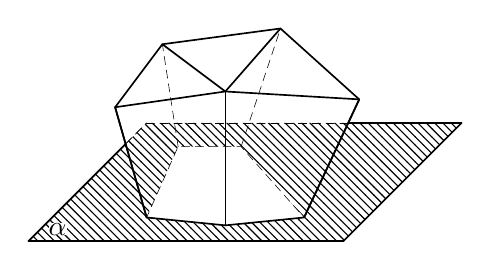
\begin{tikzpicture}[>=latex,scale=1.0]
  \tkzDefPoints{0/0/O,4/0/M,5.5/1.5/N,1.5/1.5/P}
  \tkzDefPoints{1.5/0.3/A,2.5/0.2/B,3.5/0.3/C,2.7/1.2/D,1.9/1.2/E}
  \tkzDefPoints{1.1/1.7/A',2.5/1.9/B',4.2/1.8/C',3.2/2.7/D',1.7/2.5/E'}
  \tkzInterLL(P,O)(A,A')\tkzGetPoint{F}
  \tkzInterLL(P,N)(C,C')\tkzGetPoint{G}
  \tkzDrawPolygon[draw=none,pattern=north west lines](O,M,N,P)
  \tkzDrawPolygon[densely dashed,fill=white](A,B,C,D,E)
  \tkzDrawPolygon[semithick](A',A,B,C,C',D',E')
  \tkzDrawSegments[semithick](O,M M,N N,G O,F A,A' B,B' C,C' B',C' B',A' B',D' B',E')
  \tkzDrawSegments[densely dashed](O,M M,N O,P D,D' E,E' F,P G,P)
  \tkzLabelAngle[pos=0.4,fill=white,inner sep=0pt](M,O,P){$\alpha$}
\end{tikzpicture}
\end{document}